% Appendix figures — ReCAHS paper
% \input this file AFTER the bibliography command in main.tex.
% \clearpage flushes all pending floats and forces a fresh page, so the
% appendix always begins on the page following the references.
% (IEEE-style templates use \appendices instead of \appendix — swap the
% one line below if your class requires it.)

\clearpage
\appendix
\label{sec:appendix}

This appendix collects the supporting figures: the full
$16$-cell sparsity grid (Fig.~\ref{fig:allcells}), per-cell bootstrap
confidence intervals (Fig.~\ref{fig:forest}), the diversity-source
ablation (Fig.~\ref{fig:diversity}), the PatchTST--iTransformer
degradation comparison (Fig.~\ref{fig:arch}), and the confidence-aware
fallback sweep (Fig.~\ref{fig:fallback}).

\begin{figure*}[!tp]
  \centering
  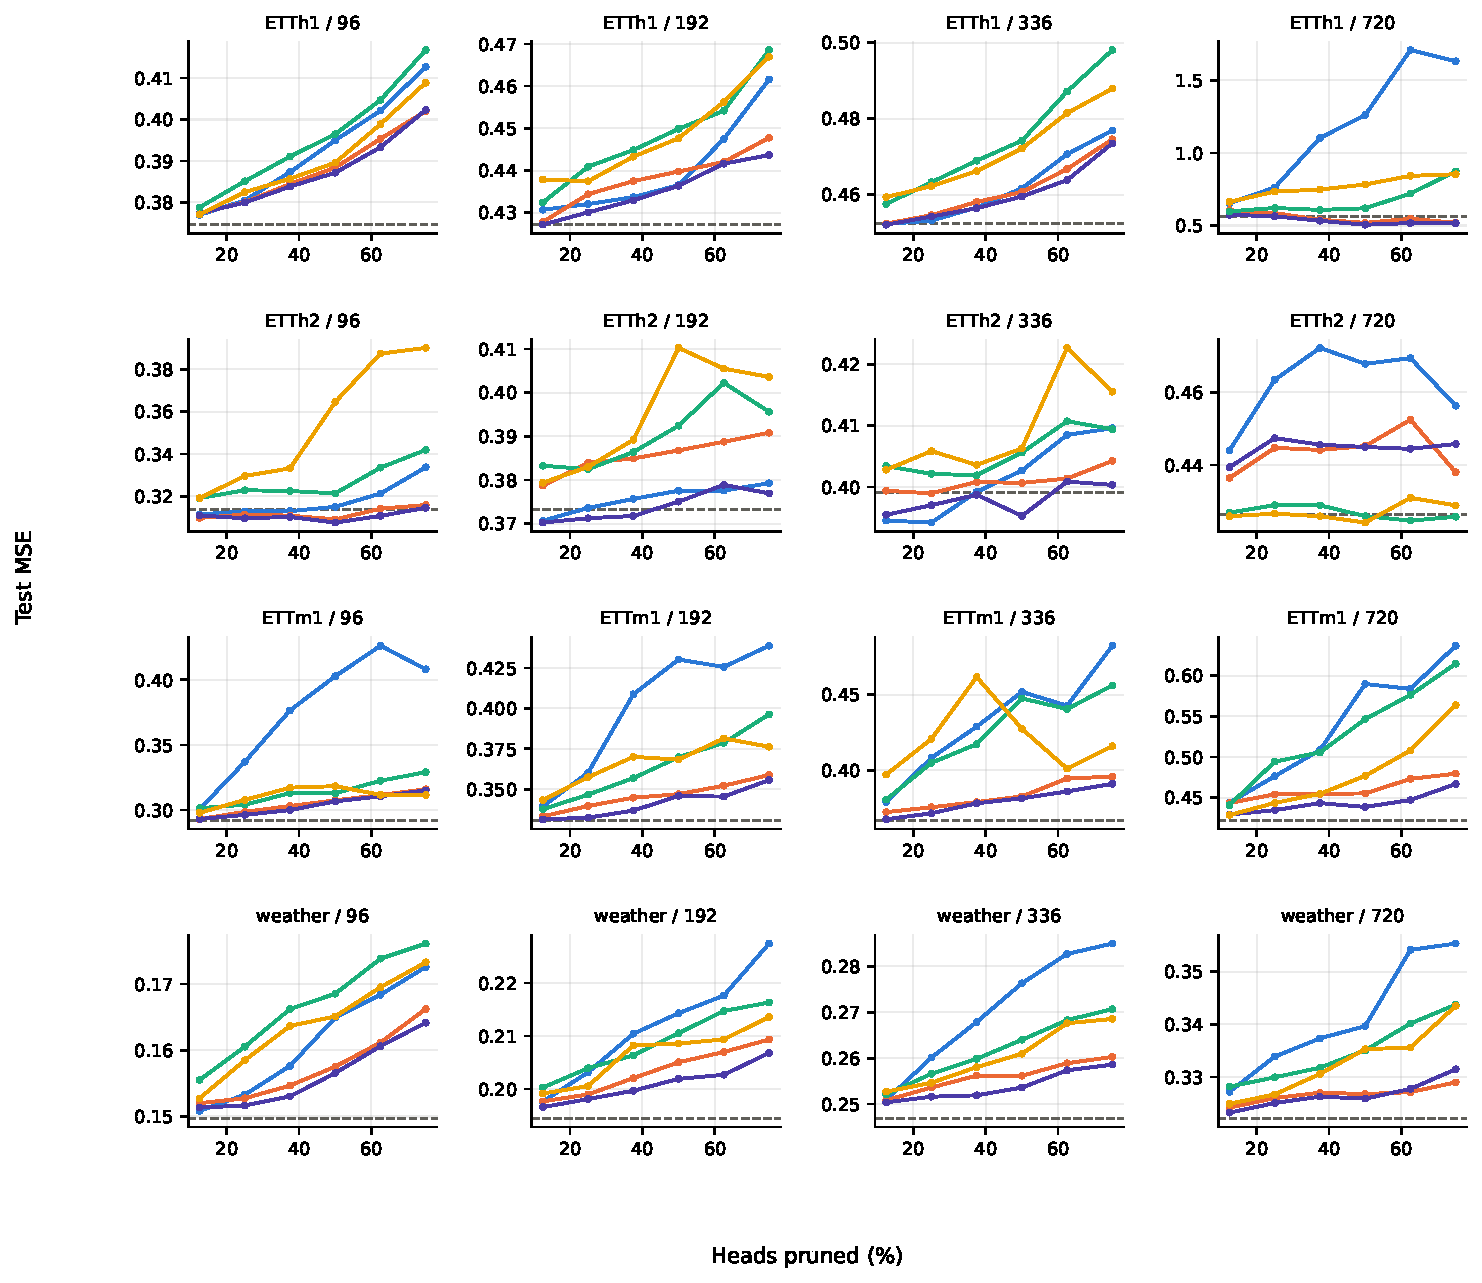
\includegraphics[width=\textwidth]{figures/fig_all_cells.pdf}
  \caption{The full grid: test MSE versus heads pruned for all 16
  dataset$\times$horizon cells (PatchTST; colors as in
  Fig.~\ref{fig:sweep}). Failures of the independent-importance ranking
  concentrate on ETTm1 and long horizons.}
  \label{fig:allcells}
\end{figure*}

\begin{figure*}[!tp]
  \centering
  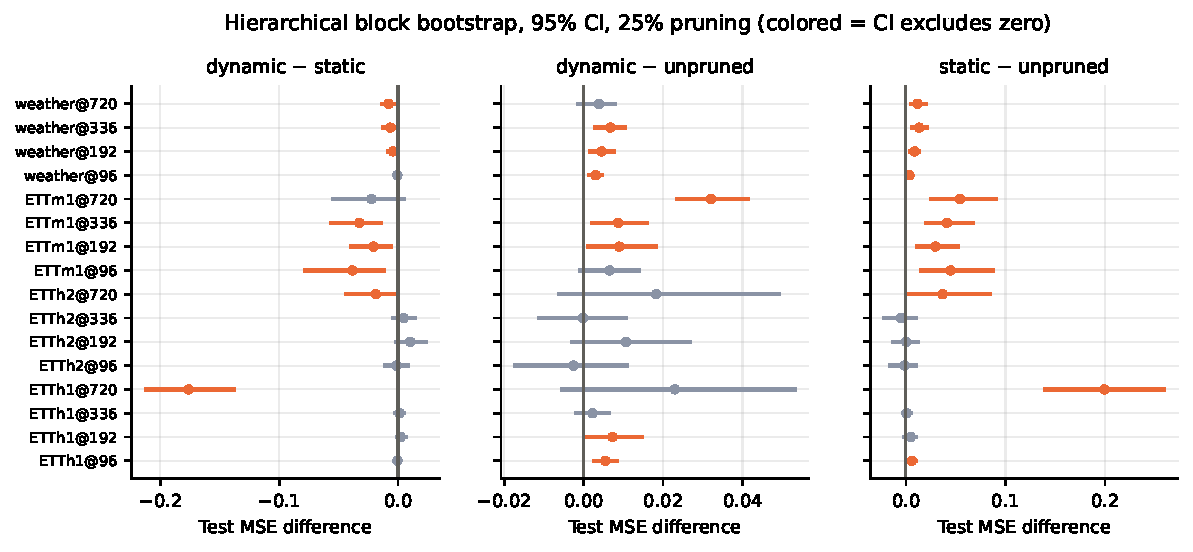
\includegraphics[width=\textwidth]{figures/fig_bootstrap_forest.pdf}
  \caption{Hierarchical circular moving-block bootstrap (seeds $\times$
  96-window blocks, $10^4$ replicates) at $25\%$ sparsity: 95\% CIs for
  paired test-MSE differences per cell. Colored intervals exclude zero.
  Dynamic is significantly better than the standard static in $8/16$
  cells and never significantly worse (left); static is significantly
  worse than the unpruned baseline in $11/16$ cells (right).}
  \label{fig:forest}
\end{figure*}

\begin{figure}[!htbp]
  \centering
  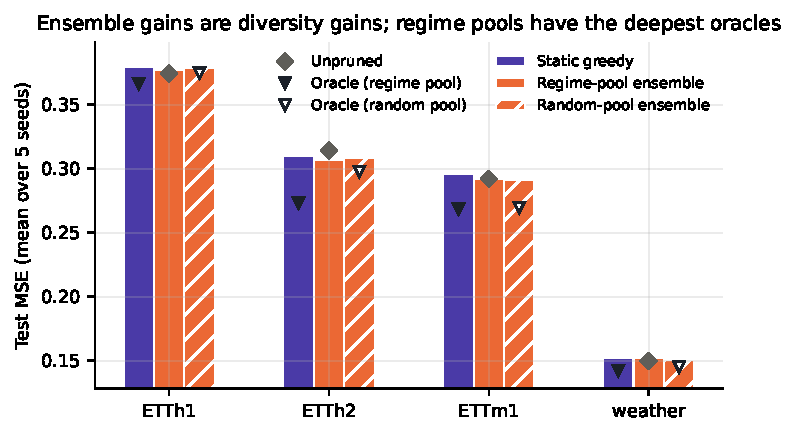
\includegraphics[width=\linewidth]{figures/fig_diversity_headroom.pdf}
  \caption{Diversity-source ablation at horizon 96. Ensembles over
  regime-partitioned pools (solid orange) and random-subsample pools
  (hatched orange) perform comparably, but regime pools yield
  systematically deeper oracles (filled vs.\ open triangles) on all four
  datasets.}
  \label{fig:diversity}
\end{figure}

\begin{figure*}[!tp]
  \centering
  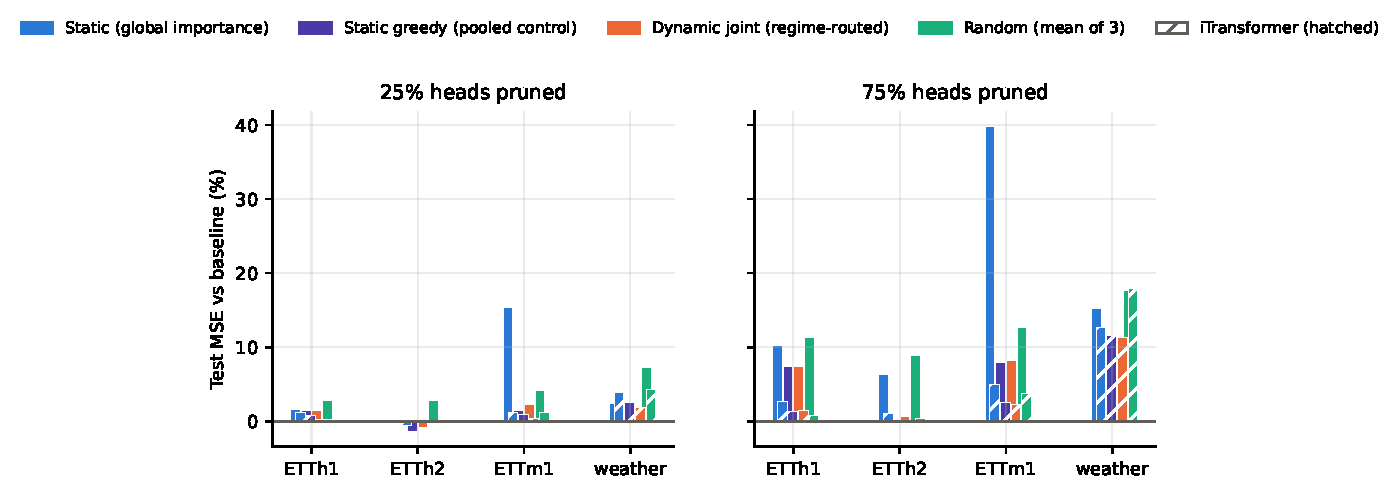
\includegraphics[width=\textwidth]{figures/fig_arch_comparison.pdf}
  \caption{Degradation at $25\%$ and $75\%$ pruning per method and
  dataset, PatchTST (solid) versus iTransformer (hatched), horizon 96.
  Cross-variate heads are substantially more redundant except on
  21-variate Weather.}
  \label{fig:arch}
\end{figure*}

\begin{figure*}[!tp]
  \centering
  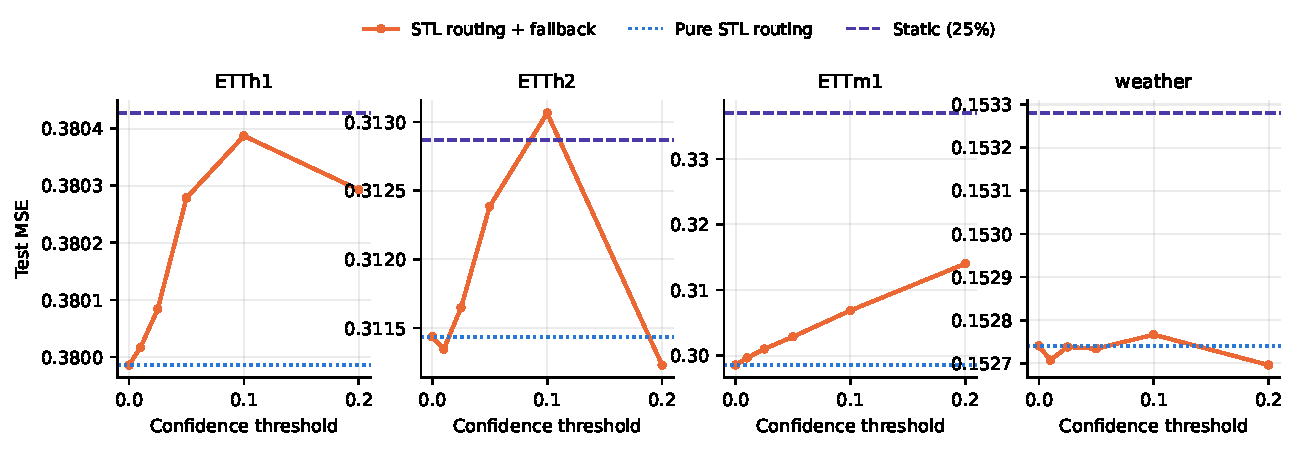
\includegraphics[width=\textwidth]{figures/fig_fallback_appendix.pdf}
  \caption{Confidence-aware fallback at $25\%$ sparsity, horizon 96:
  routing ambiguous windows (STL confidence margin below threshold) to
  the static mask never improves on pure STL routing, and inherits the
  static mask's weakness where it is fragile (ETTm1).}
  \label{fig:fallback}
\end{figure*}
